\documentclass{ximera}


\graphicspath{
  {./}
  {ximeraTutorial/}
  {basicPhilosophy/}
}

\newcommand{\mooculus}{\textsf{\textbf{MOOC}\textnormal{\textsf{ULUS}}}}


\usepackage{tkz-euclide}\usepackage{tikz}
\usepackage{tikz-cd}
\usetikzlibrary{arrows}
\tikzset{>=stealth,commutative diagrams/.cd,
  arrow style=tikz,diagrams={>=stealth}} %% cool arrow head
\tikzset{shorten <>/.style={ shorten >=#1, shorten <=#1 } } %% allows shorter vectors

\usetikzlibrary{backgrounds} %% for boxes around graphs
\usetikzlibrary{shapes,positioning}  %% Clouds and stars
\usetikzlibrary{matrix} %% for matrix
\usepgfplotslibrary{polar} %% for polar plots
\usepgfplotslibrary{fillbetween} %% to shade area between curves in TikZ
\usetkzobj{all}
\usepackage[makeroom]{cancel} %% for strike outs
%\usepackage{mathtools} %% for pretty underbrace % Breaks Ximera
%\usepackage{multicol}
\usepackage{pgffor} %% required for integral for loops



%% http://tex.stackexchange.com/questions/66490/drawing-a-tikz-arc-specifying-the-center
%% Draws beach ball
\tikzset{pics/carc/.style args={#1:#2:#3}{code={\draw[pic actions] (#1:#3) arc(#1:#2:#3);}}}



\usepackage{array}
\setlength{\extrarowheight}{+.1cm}
\newdimen\digitwidth
\settowidth\digitwidth{9}
\def\divrule#1#2{
\noalign{\moveright#1\digitwidth
\vbox{\hrule width#2\digitwidth}}}
























%%This is to help with formatting on future title pages.
\newenvironment{sectionOutcomes}{}{}


\title{Encoding Visually}


\begin{document}

\begin{abstract}
pairs to dots
\end{abstract}
\maketitle


Function notation allows us to talk about individual pairs inside a function.


\[
(d, F(d))
\]

$d$ is sitting in the left position of our ordered pair, therefore it represents a domain number. $F(d)$ represents the value of the function at $d$ and is written on the right in the ordered pair.


\begin{example}
SUppose 4 is a member of the domain of the function $H$. Then $H(4)$ represents the value of $H$ at $4$. $H(4)$ is a member of the range of $H$. $(4, H(4))$ is a pair in the function $H$.

If we happen to know that $(4, 9)$ is a pair in the funciton $H$, then we know $H(4) = 9$.

\end{example}


Aside from talking about individual pairs, we might also like to talk about the whole collection at once.  Our first attempt at this is via pictures. We need a way to visually represent a single pair and then convert all pairs to a picture.  With this picture, we can analyze the function as a whole, identify important places in the domain, detect trands in the data, quick estimate information about the whole function.


\section{Visually Encoding}

Our plan is to visually encode the pair $(d,f(d))$ as a dot in the Cartesian plane with coordinates $(d,f(d))$.

\begin{center}
That's it!!!!
\end{center}







\begin{image}
\begin{tikzpicture}
        \begin{axis}[
            domain=0:4, ymax=5, xmax=5, ymin=-5, xmin=-5,
            axis lines =center, xlabel=$x$, ylabel=$y$,
            every axis y label/.style={at=(current axis.above origin),anchor=south},
            every axis x label/.style={at=(current axis.right of origin),anchor=west},
            axis on top,
          ]
          
        \addplot [color=penColor2,only marks,mark=*] coordinates{(3,2)};


        \draw[decoration={brace,raise=.2cm,mirror},decorate,thin] (axis cs:3.05,0)--(axis cs:3.05,2);
        \draw[decoration={brace,raise=.2cm},decorate,thin] (axis cs:0,2.05)--(axis cs:3,2.05);
        \node[anchor=east] at (axis cs:1.85,3) {$d$};
        \node[anchor=east] at (axis cs:4.5,1) {$f(d)$};
                     
        \node at (axis cs:4,2.7) [penColor] {$(d,f(d))$};

        \end{axis}
\end{tikzpicture}
\end{image}




\begin{example}

The fact that $f(3)=2$ for the function $f$, is encoded with a dot at $(3, 2)$.

\begin{image}
\begin{tikzpicture}
\begin{axis}[
            domain=0:4, ymax=5, xmax=5, ymin=-5, xmin=-5,
            axis lines =center, xlabel=$x$, ylabel=$y$,
            every axis y label/.style={at=(current axis.above origin),anchor=south},
            every axis x label/.style={at=(current axis.right of origin),anchor=west},
            axis on top,
          ]
        
          \addplot [color=penColor2,only marks,mark=*] coordinates{(3,2)};


          \draw[decoration={brace,raise=.2cm,mirror},decorate,thin] (axis cs:3.05,0)--(axis cs:3.05,2);
          \draw[decoration={brace,raise=.2cm},decorate,thin] (axis cs:0,2.05)--(axis cs:3,2.05);
          \node[anchor=east] at (axis cs:1.85,3) {$3$};
          \node[anchor=east] at (axis cs:4,1) {$2$};
                    
          
          \node at (axis cs:3.7,2.7) [penColor] {$(3,2)$};

        \end{axis}
\end{tikzpicture}
\end{image}

\end{example}



\begin{example}
Here is a graph of $y=H(t)$. Which point represents $H(-3) = -2$?
\begin{image}
\begin{tikzpicture}
\begin{axis}[
            domain=0:4, ymax=5, xmax=5, ymin=-5, xmin=-5,
            axis lines =center, xlabel=$t$, ylabel=$y$,
            every axis y label/.style={at=(current axis.above origin),anchor=south},
            every axis x label/.style={at=(current axis.right of origin),anchor=west},
            axis on top,
          ]

          
        \addplot [color=penColor2,only marks,mark=*] coordinates{(-3,2)};
        \addplot [color=penColor2,only marks,mark=*] coordinates{(3,-2)};
        \addplot [color=penColor2,only marks,mark=*] coordinates{(-3,-2)};
        \addplot [color=penColor2,only marks,mark=*] coordinates{(3,2)};

        \node at (axis cs:-3.4,2.4) [penColor] {$A$};
        \node at (axis cs:3.4,2.4) [penColor] {$B$};
        \node at (axis cs:-3.4,-2.4) [penColor] {$C$};
        \node at (axis cs:3.4,-2.4) [penColor] {$D$};

\end{axis}
\end{tikzpicture}
\end{image}


\begin{multipleChoice}
\choice {$A$}
\choice {$B$}
\choice[correct] {$C$}
\choice {$D$}
\end{multipleChoice}

\end{example}



\begin{example}
Suppose $k$ is a funnction with $k(-1)>0$, then which quadrant will its corresponding dot be plotted?
\begin{image}
\begin{tikzpicture}
\begin{axis}[
            domain=0:4, ymax=5, xmax=5, ymin=-5, xmin=-5,
            axis lines =center, xlabel=$t$, ylabel=$y$,
            every axis y label/.style={at=(current axis.above origin),anchor=south},
            every axis x label/.style={at=(current axis.right of origin),anchor=west},
            axis on top,
          ]

        
        \node at (axis cs:3.4,2.4) [penColor] {$I$};
        \node at (axis cs:-3.4,2.4) [penColor] {$II$};
        \node at (axis cs:-3.4,-2.4) [penColor] {$III$};
        \node at (axis cs:3.4,-2.4) [penColor] {$IV$};

\end{axis}
\end{tikzpicture}
\end{image}


\begin{multipleChoice}
\choice {$I$}
\choice[correct] {$II$}
\choice {$II$}
\choice {$IV$}
\end{multipleChoice}

\end{example}



Graphs of functions are just a collection of a bunch of dots (a curve).  Each dot represents a pair in the function.  Each dot has two coordinates.  The horizontal (first) coordinate is the domain number and the vertical (Second) coordinate is the function value at that domain value.

The functions we are most interested in have milloions and billions of trillions of dots.  They get very difficult to see when bumped up against each other.  Pretty soon your eyes get tricked into seeing an object.



\begin{image}
\begin{tikzpicture}
  \begin{axis}[
            domain=-4:4, ymax=5, xmax=4, ymin=-5, xmin=-4,
            axis lines =center, xlabel=$x$, ylabel=$y$,
            every axis y label/.style={at=(current axis.above origin),anchor=south},
            every axis x label/.style={at=(current axis.right of origin),anchor=west},
            axis on top,
          ]
          
    \addplot [draw=penColor2,very thick,smooth] {(x+1)*(x-3)};
    \node at (axis cs:1,3) [penColor2] {$y=(x+1)(x-3)$};
           

  \end{axis}
\end{tikzpicture}
\end{image}




\begin{image}
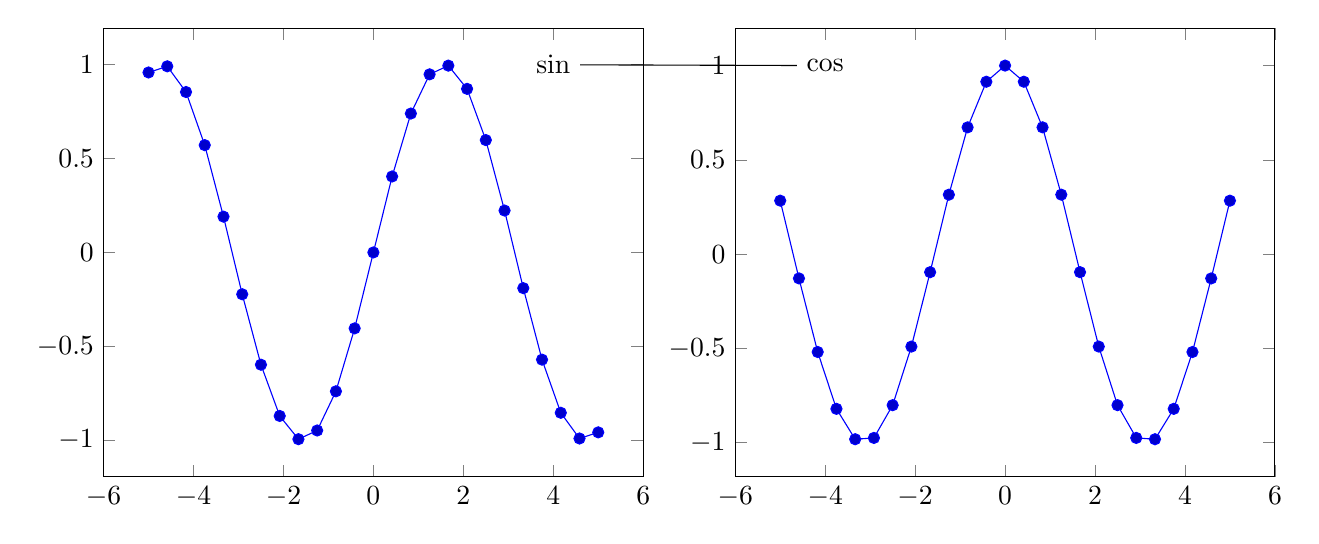
\begin{tikzpicture}
    \begin{axis}[name = sinax]
        \addplot {sin(deg(x))};
        \node (sin) at (axis cs:4,1) {sin};
    \end{axis}
    \begin{axis}[at={(sinax.outer east)},anchor=outer west]
        \addplot {cos(deg(x))};
        \node (cos) at (axis cs:-4,1) {cos};
    \end{axis}

\draw (cos) -- (sin);

\end{tikzpicture}
\end{image}























Of course, our functions will have more than four points, because their domains are going to include intervals of the real numbers.






\end{document}
